%!TEX root =  ../thesis.tex
% CHAPTER 1
\chapter{Introduction}
\label{chp:b1}

Lorem ipsum dolor sit amet, consectetur adipiscing elit. Quisque vel maximus dolor. Nunc ex ex, eleifend vel lacus a, lobortis iaculis turpis. Phasellus eget nibh facilisis urna interdum tincidunt. Donec finibus leo vel mi eleifend, ut suscipit augue sodales. Etiam eu faucibus nulla. Cras sed vulputate erat, ac placerat eros. In hac habitasse platea dictumst. Quisque tincidunt tortor eu nisl pretium aliquet. Praesent elementum est risus, ut faucibus quam efficitur et. Suspendisse varius dui quis ipsum commodo convallis. Donec congue, felis ut tempus vestibulum, nulla nisi euismod orci, ut iaculis dolor turpis id felis. Sed semper pulvinar ipsum, a ultricies enim ultrices nec. Maecenas a urna non dolor gravida tincidunt.

Pellentesque habitant morbi tristique senectus et netus et malesuada fames ac turpis egestas. Nullam porttitor lacus sed orci mattis, ut pulvinar ex euismod. Mauris consectetur turpis id dui gravida, quis interdum dui pulvinar. Vestibulum at ullamcorper nisl. Suspendisse ullamcorper lacus ut tempus porta. Duis ligula dolor, tincidunt rutrum arcu ac, semper ornare ante. Phasellus id facilisis libero, quis vehicula ante. Donec lorem eros, facilisis a diam in, laoreet aliquam elit. \parencite{aaltonenHowWeMake2005}.
	

	\begin{figure}[h!]
			\centering
			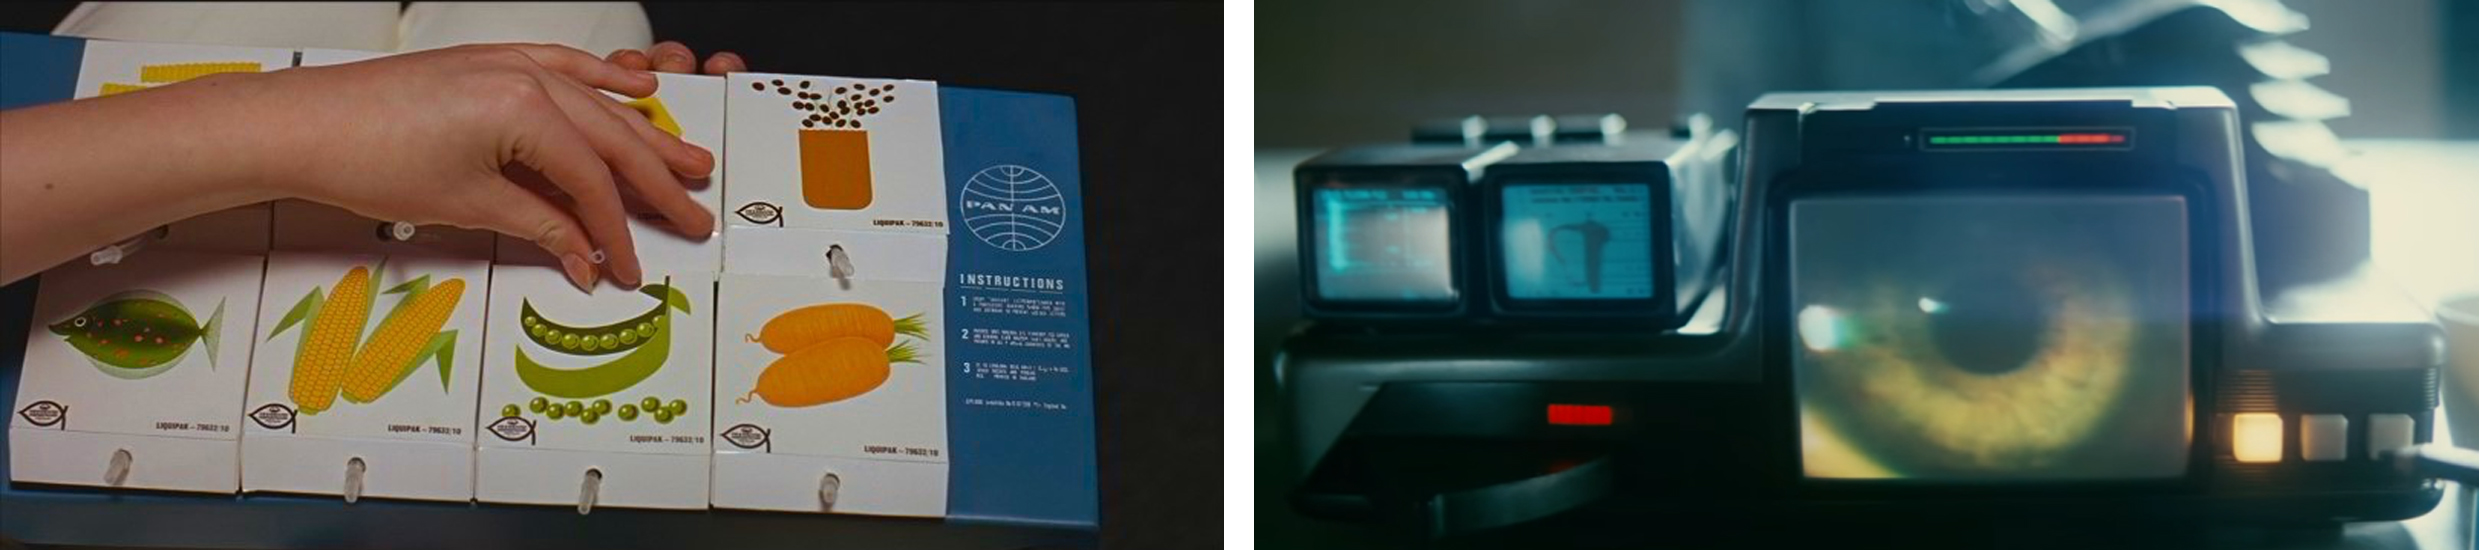
\includegraphics[width=.8\textwidth]{figures/2001-Bladerunner.jpg}
			\caption{Screencaps from a movie \parencite{bladeRunner}.}
			\label{fig:movies}
	\end{figure}

	\begin{comment}
		A comment here that will not appear in the thesis.
	\end{comment}


	

\section{Research Questions and Approach}
\label{Research Questions}
	Lorem ipsum dolor sit amet, consectetur adipiscing elit. Quisque vel maximus dolor. Nunc ex ex, eleifend vel lacus a, lobortis iaculis turpis. Phasellus eget nibh facilisis urna interdum tincidunt. Donec finibus leo vel mi eleifend, ut suscipit augue sodales. Etiam eu faucibus nulla. Cras sed vulputate erat, ac placerat eros. In hac habitasse platea dictumst. Quisque tincidunt tortor eu nisl pretium aliquet. Praesent elementum est risus, ut faucibus quam efficitur et. Suspendisse varius dui quis ipsum commodo convallis. Donec congue, felis ut tempus vestibulum, nulla nisi euismod orci, ut iaculis dolor turpis id felis. Sed semper pulvinar ipsum, a ultricies enim ultrices nec. Maecenas a urna non dolor gravida tincidunt.


\section{Structure of the Thesis}
	This thesis consists of Chapter~\ref{chp:b2} (p.~\pageref{chp:b2}), and Chapter~\ref{chp:b3} (p.~\pageref{chp:b3}). 